\section{Fundamentos Técnicos}

% --- Ponente 2 ---

\begin{frame}{El Autoencoder Variacional (VAE)}
 \begin{figure}
     \centering
     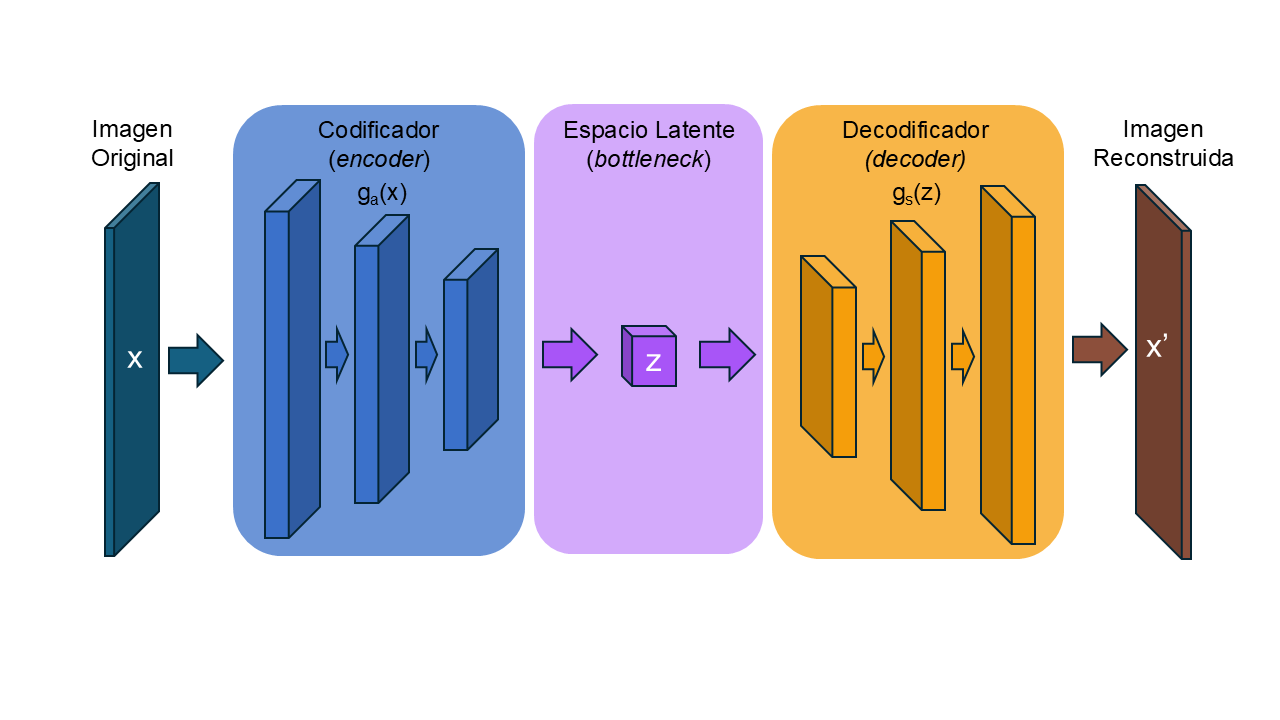
\includegraphics[width=0.9\textwidth]{images/diagrama_autoencoder}
     \caption{Arquitectura del Autoencoder Variacional para NIC.}
 \end{figure}
\end{frame}

\begin{frame}{El Compromiso Tasa-Distorsión}
\begin{alertblock}{Función de pérdida fundamental}
$$L = R + \lambda \cdot D$$
\end{alertblock}
\begin{itemize}
    \item $R$ (\textit{Rate}): Número de bits necesarios para codificar la representación latente.
    \item $D$ (\textit{Distortion}): Error de reconstrucción (calidad perdida).
    \item $\lambda$: Parámetro que \textbf{equilibra} compresión vs. calidad.
\end{itemize}
\vspace{0.3cm}
Un $\lambda$ alto prioriza calidad; un $\lambda$ bajo prioriza compresión.
\end{frame}

\begin{frame}{El Reto de la Cuantización}
\begin{itemize}
    \item La cuantización (redondeo a enteros) es \textbf{necesaria} para obtener un bitstream discreto.
    \item Problema: crea una función escalera con \textbf{gradiente nulo} $\rightarrow$ rompe la retropropagación.
\end{itemize}
\begin{exampleblock}{Solución: Ruido uniforme aditivo}
Durante el entrenamiento, se sustituye el redondeo por \textbf{inyección de ruido uniforme} $\mathcal{U}(-0.5, 0.5)$, creando un sustituto diferenciable.
\end{exampleblock}
\begin{itemize}
    \item En inferencia se usa el redondeo real.
    \item Permite entrenar el sistema end-to-end con descenso de gradiente.
\end{itemize}
\end{frame}
